%TODO
%
%++ 186 positionen checken
%-- leungting buch durcharbeiten
%+ korrekturlesen
%
%
%++ boxen hinzu
%	korrektheit pruefen:
%		S1 tan "von unten raus" uebung mit partner (lehrer vom 5.)
%		S2, ausgestreckter fauststoss soll von partner von vorne draufschlagbar sein, stabil bleiben, %kraft nach unten leiten
%		S3, im spiegel nur kleiner finger sichtbar
%		S4, partner hebt beim lansao von unten nach oben an, bzw zieht/drueckt (selbiges beim djam-sao)
%		S6, zweiten tan hinzu, soll mitte besetzt sein
%		S7, bongsao muss mit sehenspannung arbeiten, hand dabei ganz locker
%		DONE S6, dai-cheung zweiten hinzu
%	gaengige fehler
%		S1	* tan zu hoch, zu spitzer winkel
%			* nicht mit elle schneiden beim gan
%		generell: beim schlusssequenz huensao wird arm gebeugt
%		S2&co: schulter geht nach vorne
%		S4	* lansao zu weit oben
%		S7, bongsao geht schulter hoch
%		S8, drei bewegungen werden nicht gleichzeitig ausgefuehrt
		

\section{Siu-Nim-Tau}
%%%%%%%%%%%%%%%%%%%%%%%%%%%%%%%%%%%%%%%%%%
%%%%%%%%%%%%%%%%%%%%%%%%%%%%%%%%%%%%%%%%%%
% http://everything2.com/title/Sil+Lum+Tao


\WTMediaInclude{\WTMediaRefSNT}{Die Siu-Nim-Tau vorgef\"uhrt von Yip Man}{1:22}


Siu-Nim-Tau (SNT) bedeutet so etwas wie \quoteit{kleine Idee} oder auch \quoteit{kleine Ideen Form}. Sie wird deshalb als klein bezeichnet, da man recht \textbf{isolierte Bewegungen} ausf\"uhrt und sich auf das Kleine, die Details konzentriert. So gibt es in dieser Form z.B. keinerlei Wendungen oder Schritte, der Oberk\"orper und die Beine bleiben durchgehend in der selben Position und bewegen sich nicht, sondern einzig die Arme und H\"ande f\"uhren die Aktionen aus.

Ziel ist es hier \textbf{f\"ur den Anf\"anger} lernen sich zu entspannen, seine Schultern unten zu lassen und locker sein. Weiters wird einem das \textbf{Finden der K\"orpermitte} antrainiert. So legt man z.B. sehr viel Wert auf das korrekte Zur-Mitte-Stellen der Faust im 2.~Satz, oder auch das Zur\"uckziehen des seitlichen Pak-Saos im 3.~Satz zur Zentrallinie. Auf der anderen Seite wird auch das \textbf{K\"orperende} aufgezeigt, so dass die Techniken nicht weiter nach Au{\ss}en als die Schulter (seitlicher Pak-Sao im 3. und 5.~Satz), nicht weiter nach unten als der Genitalbereich (Gam-Sao im 4.~Satz) oder h\"oher als das Ohr (Lau-Sao im 6.~Satz) gehen sollen. Es bildet sich damit ein Rechteck dass den K\"orper von Au{\ss}en und Innen trennt und in dessen Mitte sich die Zentrallinie befindet.
% TODO reference zum zentrallinien konzept


\begin{WTCommonBegriff}
	Die \textbf{Siu-Nim-Tau} (SNT) wird in manchen Stilen auch \textbf{Siu-Lin/Lim-Tau} (SLT) geschrieben, was dann soviel bedeutet wie \quoteit{ein bisschen am Anfang \"uben}. Und nicht genug, es gibt auch die Bezeichnung \textbf{Siu-Lam-Tau}, \quoteit{Vergiss nicht, dass der Ursprung des Wing Chun im Shaolin liegt}.
\end{WTCommonBegriff}


% TODO wie schreibt man dim-dim-chin ?
\textbf{Das Motto} der SNT lautet \textit{Punkt-Punkt-Klar}, es sollen also alle Stationen (Punkte) der Bewegungen klar sichtbar durchlaufen werden. Eine \"ubereilige und schlampige Ausf\"uhrung ist also nicht angebracht und verf\"alscht den Ablauf. Weiters gilt es die ganze Zeit \"uber folgende Mottos, entnommen aus \cite{WTBIBLeu11}, zu beachten:

\begin{itemizeNarrow}
	\item Dr\"ucke deinen Kopf Richtung Himmel und stehe fest am Boden.
	\item Kopf hoch mit horizontalem Blick.
	\item Aufnahmef\"ahiger Brustkorb und aufgerichteter R\"ucken.
	\item H\"ufte gerade und Bauch einziehen.
	\item Bei allen Bewegungen der Arme zu beachten: Tiefer Ellbogen und entspannte Schulterhaltung.
	\item Wenn eine Armbewegung erfolgt: Schau in die Richtung der Handbewegung.
\end{itemizeNarrow}




\subsection*{Die acht S\"atze im \"Uberblick}

Die Betitelung der einzelne S\"atze ist eine pers\"onliche Merkhilfe und Versch\"onerung welche gerne in anderen Kampfk\"unsten auch vorgenommen werden, die aber so im Unterricht der EWTO \textit{nicht anzufinden} ist. Vielmehr werden dort die S\"atze einfach anhand ihrer Nummerierung 1-8 benannt.

\begin{flushleft}
\WTKurzSatz{1}{Schneidende Arme}{Es \"uberkreuzen beide Arme vor dem K\"orper, schneiden anschlie{\ss}end gerade runter, rollen nach innen zur urspr\"unglichen Position und ziehen zur\"uck.}
\WTKurzSatz{2}{Einfacher Fauststo{\ss}}{Die Faust stellt sich vorbereitend in die K\"orpermitte und schl\"agt gerade nach vorne; selbiges wird auf der rechten Seite wiederholt.}
\WTKurzSatz{3}{Dreifache Verehrung}{Dieser (f\"ur gew\"ohnlich seeehr langsam ausgef\"uhrte) Satz wiederholt den mittleren Teil dreimal; die aufgestellte Handfl\"ache erinnert dabei an die Haltung eines M\"onches.}
\WTKurzSatz{4}{Lange Br\"ucke}{Der l\"angste (im Sinne von \quote{meiste Techniken enthaltende} Satz startet mit ein paar Handfl\"achenst\"osse und besitzt rein nur doppelt ausgef\"uhrte Bewegungen.}
\WTKurzSatz{5}{Mit der offenen Hand schlagen}{Hier werde nur kurz zur Seite geschlagen und anschlie{\ss}end zur Seite, beides mit offenen Handfl\"achen.}
\WTKurzSatz{6}{Ein D malen}{Zwei Techniken von diesem Satz, n\"amlich der halbkreisf\"ormig wischende Kwat-Sao und der gerade nach oben f\"uhrende Lau-Sao, erinnern an die Form eines \texttt{D}.}
\WTKurzSatz{7}{Schwingen ausbreiten}{Dieser Satz startet mit einem Bong-Sao, \"ubersetzt mit Fl\"ugel- oder Schwingen-Arm, und f\"uhrt \"uber den \"ahnlich gestellten Tan-Sao zu einem Handfl\"achenstoss.}
\WTKurzSatz{8}{Befreiungssatz}{Im letzten Teil wird eine einarmige Griffbefreiung ge\"ubt, dreimal, mit anschlie{\ss}enden Kettenfaustst\"osse, ebenfalls drei an der Zahl.}
\end{flushleft}

\begin{flushleft}
	\textbf{Achtung: } In den folgenden Abbildungen sind s\"amtliche \textbf{seitengleiche S\"atze nur einmal f\"ur links} dargestellt, da sich die rechte Seite recht schnell selbst herausfinden lassen sollte und es klarerweise auch platzsparender so ist. Nicht betroffen sind nat\"urlich davon die S\"atze bei denen beide Arme zum Einsatz kommen, n\"amlich der 1., 4. und 8.~Satz.
\end{flushleft}


\begin{WTSatz}{Schneidende Arme}% 1. SATZ
%%%%%%%%%%%%%%%%%%%%%%%%%%%%%%%%%%%%%%%%%%

	\WTSatzTechniken{Tan-Sao, Gan-Sao}

	\begin{WTSatzTeil}{Gau-Cha-Tan-Sao}{Gekreuzte Handfl\"achen nach oben H\"ande}
		\WTGalerySlideshowFour{siunimtau/1/1}{siunimtau/1/2}{siunimtau/1/3}{siunimtau/1/3b}
		
		Als allererstes werden beide geschlossene F\"auste a) ganz ge\"offnet sodass die Handfl\"achen eine gerade Oberfl\"ache bilden b). Danach werden die H\"ande, gef\"uhrt von den Ellbogen (welche zu der Zeit bereits eine gewisse Vorspannung besitzen) nach vorne geschoben c) bis dass ein Abstand von einer Faust breit zwischen K\"orper und Ellbogen besteht, und die Fingerspitzen auf H\"ohe der Schultern sind d). Um korrekte Winkeln zu gew\"ahrleisten sollte noch gepr\"uft werden, ob die Hautlinien beim rechten Handgelenk gerade noch sichtbar sind, und die Ellbogen seitlich mit dem K\"orper abschliessen.
		
		Der sogenannte \textit{gekreuzte Tan-Sao} ist in beidh\"andiger Ausf\"uhrung nur in der Form zu sehen, da er wenn dann nur einarmig und in gewendeter Position Anwendung findet. Man kann dies ganz einfach nachpr\"ufen in dem man eine Hand wegnimmt, und eine Wendung durchf\"uhrt.
		
		%TODO bild von einarmig-gekreuzten tan sao in wendung
		%TODO bild von hautlinie die gerade mit hand abschliesst fuern gekreuzten-tan sao
	\end{WTSatzTeil}
	
	\begin{WTSatzTeil}{Gau-Cha-Gan-Sao}{Gekreuzte schneidende Arme}
		\WTGalerySlideshowTwo{siunimtau/1/3}{siunimtau/1/4}
		
		Startend im doppelten Tan-Sao e) schneidet der Gan-Sao (nicht zu verwechseln mit dem Gam-Sao) mit der Elle eine gerade Linie hinunter f), so als w\"urden die Arme etwas abschneiden wollen, und beschreibt \textbf{nicht} in einer Wischbewegung einen Kreis! Darum wird auch geraten die Bewegung nicht bewusst zu steuern, sondern einfach nur die Arme locker fallen lassen. Am Ende wird der Unterarm leicht nach au{\ss}en routiert so dass man auch wirklich mit dem Knochen auftrifft.
	\end{WTSatzTeil}
	
	\begin{WTSatzTeil}{Kwan-Sao}{Rotierender Arm}
		\WTGalerySlideshowThree{siunimtau/1/4}{siunimtau/1/5}{siunimtau/1/6}
		
		Ausgehend vom fertigen Gan-Sao g) werden die Arme nach oben rotiert h), wobei die H\"ande nahe am K\"orper entlang angehoben werden. Der linke Arm dreht sich dabei unter dem Rechten durch und befindet sich dann weiter innen.
		
		Am Schluss der Bewegung befindet man sich exakt wieder in der urspr\"unglichen Tan-Sao Position i) mit der linken Hand oben.
		
		\begin{WTCommonNoob}
			Beim Kwan-Sao werden Handgelenke nicht abgewinkelt, sondern bleiben eine geradlinige Verl\"angerung des Unterarms. Um Platz zu machen f\"uhr die L\"ange der Arme muss man die \textbf{Ellb\"ogen} leicht \textbf{nach aussen} schieben.
		\end{WTCommonNoob}
	\end{WTSatzTeil}
	
	\begin{WTSatzTeil}{Sao-Kuen}{Ellbogen nach Hinten}
		\WTGalerySlideshowThree{siunimtau/1/6}{siunimtau/1/7}{siunimtau/1/8}
		
		Ausgehend vom Tan-Sao j) wird mit beiden H\"anden gleichzeitig eine Faust gemacht k) und dann stossen die Ellb\"ogen dynamisch nach hinten, sodass die F\"auste wieder auf Brusth\"ohe sind l). % TODO heisst wie schreibt man Sao Chong??
		%Dieser Teil kann einerseits verstanden werden als das nach hinten stellen der F\"auste (Kuen) bis zur Brust, oder andererseits mit mehr Betonung auf die Ellbogen die zur\"uck ziehen, also einem Sao Chong.
	\end{WTSatzTeil}
	
\end{WTSatz}

%%%%%%%%%%%%%%%%%%%%%%%%%%%%%%%%%%%%%%%%%%

\begin{WTSatz}{Einfacher Fauststo{\ss}}% 2. SATZ
	
	\WTSatzTechniken{Chung-Kuen}
	
	\begin{WTSatzTeil}{Yat-Gee-Chung-Kuen}{Fauststoss}
		\WTGalerySlideshowFour{siunimtau/2/1}{siunimtau/2/2}{siunimtau/2/3}{siunimtau/2/4}
		
		Am Anfang des zweiten Satzes a) wird, noch bevor etwas anderes passiert, die linke Faust an ihrem Platz in die Vertikale gedreht b). Nun besetzt die Faust nahe am K\"orper die Zentrallinie c) wobei die Auftreffsfl\"ache schon gerade nach vorne zeigt. Zu guter Letzt wird der Arm gestreckt d) in dem der Ellbogen die Bewegung anf\"uhrt. Der Schlag soll nicht verkrampft ausgef\"uhrt werden, als auch kein Bizeps kommt zum Einsatz. Stattdessen spannt der K\"orper nur ganz am Anfang der Bewegung und ganz kurz vor dem Aufschlag; w\"ahrend der \textit{Flugzeit} ist der Arm locker. Auch die Kraft kommt mehr vom Trizeps und dem R\"ucken, wobei auch gerne der Lat bewusst \"uberm\"a{\ss}ig angespannt sein kann um ein Mitgehen der Schulter zu verhindern.
		
		Diese \"Ubung soll einem zeigen wo sich eigentlich seine Mitte befindet. Die Siu Nim Tau zeigt einem damit die Grundlagen und Positionen von seinem K\"orper. Man lernt quasi sich selbst einmal kennen, um dann sp\"ater auch andere kennen zu lernen $;)$
		
	\begin{WTCommonBegriff}
		Die im WT verwendete vertikale Faust wird im Chinesischen auch als \textit{Sonnenzeichen-Faust} bezeichnet, da das Symbol f\"ur Sonne den Konturen der Faust sehr \"ahnlich sieht:
		
		\center{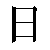
\includegraphics[width=1cm]{resources/graphics/chinese_sun_symbol}}
		\flushleft
		
		Die Aneinanderreihung von mehreren Sonnenzeichen-F\"austen ist eine Spezialit\"t im WT und wird als \textit{Ketten-Faustst\"osse} bezeichnet.
	\end{WTCommonBegriff}
			
		% TODO referenz hinzu: Siehe Anatomie des Fauststoss.
		
		% TODO pruefung stoss von vorne auf faust, a la gernot
		
	\end{WTSatzTeil}
	\begin{WTSatzTeil}{Tan-Sao, Huen-Sao, Sao-Kuen}{Handfl\"ache-oben Hand, Zirkelnde Hand, Ellbogenstoss}
	
		Diese \textbf{Schlusssequenz}\index{Schlusssequenz} findet sich am Ende von (fast) jedem Satz und besteht aus folgende f\"unf Bewegungen:
		
		
		\WTGalerySlideshowThree{siunimtau/2/5}{siunimtau/2/6}{siunimtau/2/7}
		
		
		Ausgangspunkt ist ein Tan-Sao e) von dem aus die Finger einklappen und die Spitzen den Unterarm greifen wollen f). Danach folgt eine halbe Umdrehung der Hand (Huen-Sao) g) bis mindestens ganz nach unten; eine Drehung weiter nach aussen w\"urde zu einer zus\"atzlichen Dehnung f\"uhren und simuliert somit eventuell besser das folgende Greifen im n\"achsten Schritt h).
		
		\WTGalerySlideshowThree{siunimtau/2/8}{siunimtau/2/9}{siunimtau/2/10}
		
		Ob nun zuerst die Faust gedreht wird i) oder zeitgleich mit dem Zur\"uckziehen ist mehr eine pers\"onliche Preferenz und kann von Lehrer zu Lehrer unterschiedlich sein.
		
		Wichtig ist hierbei den Arm durchgehend bei jeder Bewegung \textbf{durchgestreckt} zu lassen und nicht abzuwinkeln.
		
	\end{WTSatzTeil}
\end{WTSatz}

%%%%%%%%%%%%%%%%%%%%%%%%%%%%%%%%%%%%%%%%%%

\begin{WTSatz}{Dreifache Verehrung}% 3. SATZ
	
	\WTSatzTechniken{Tan-Sao, Huen-Sao, Wu-Sao, Fook-Sao, Pak-Sao}
	
	Der dritte Satz ist (gemeinsam mit dem vierten) der l\"angste Satz der Form. Noch dazu kommt, dass die Ausf\"uhrung vergleichsweise langsam von statten geht und die Armbewegung synchron mit der Atmung sein soll.
	
	\begin{WTSatzTeil}{Tan-Sao}{Handfl\"ache-oben Hand}
		\WTGalerySlideshowFour{siunimtau/3/1}{siunimtau/3/2}{siunimtau/3/3}{siunimtau/3/4}
		
		Von der Grundstellung aus a) wird die linke Handfl\"ache ge\"offnet b) und nahe am K\"orper entlang zur Mitte bewegt. Von dort schl\"angelt sich die Hand weiter geradlinig nach vorne c), so als ob ein Hindernis \"ueberwunden werden m\"usste, bis die Tan Sao Endposition erreicht ist d). Die offene Handfl\"ache des Tan-Sao ist hierbei komplett gerade und parallel zum Boden, der Daumen anliegend.
% TODO grafik reingeben, wo stange ist und handbewegung eingezeichnet wie drumherum bewegt wird
		
	\end{WTSatzTeil}
	\begin{WTSatzTeil}{Huen-Sao}{Zirkelnde Hand}
		\WTGalerySlideshowFour{siunimtau/3/5}{siunimtau/3/6}{siunimtau/3/7}{siunimtau/3/8}
		
		Nun werden die Fingerspitzen nach Oben zu sich gezogen e) und von der Position aus ein Halbkreis nach rechts beschrieben f). Unten angekommen stellt die Hand sich nach vorne hin \textit{Finger f\"ur Finger} auf, bis eine Sperre im Handgelenk ein Weiterdrehen unm\"oglich macht g). Erst dann wird der Ellbogen etwas nach au{\ss}en gedreht sodass die Handfl\"ache kerzengerade nach Oben zeigt h). Es gilt hierbei zu beachten dass man im Spiegel nur den kleinen Finger sieht und sich alle anderen Finger quasi dahinter verstecken. Auch kann man die letzte Drehbewegung etwas mit der Handkante betonen um diesen speziellen Angriff zu trainieren.
		
		\begin{WTCommonBegriff}
			Da es sich hier nur um eine halbe, und keine ganze Drehung handelt, wird diese Bewegung eigentlich genauer als \textit{Bon Huen Sao}\index{Huen Sao!Bon Huen Sao} (halb kreisende Hand) bezeichnet.
		\end{WTCommonBegriff}

	\end{WTSatzTeil}
	\begin{WTSatzTeil}{Wu-Sao}{Sch\"utzende Hand}
		\WTGalerySlideshowTwo{siunimtau/3/8}{siunimtau/3/9}
		
		Mit aufgestellter Hand i) zieht man nun den Arm nach Hinten, so dass die Hand ungef\"ahr eine Faust vom K\"orper entfernt stehen bleibt j). Die Konzentration ist dabei beim geradlinig nach hinten ziehenden Ellbogen, von dem aus die Bewegung angesteuert wird.
		
	\end{WTSatzTeil}
	\begin{WTSatzTeil}{Fook-Sao, Huen-Sao, Wu-Sao x3}{Br\"uckenarm, Zirkelnde und Sch\"utzende Hand}
		\WTGalerySlideshowFour{siunimtau/3/9}{siunimtau/3/10}{siunimtau/3/11}{siunimtau/3/6}
		
		Der folgende Abschnitt stellt die eigentliche Verehrung dar und wird gezeigt in dem man \textbf{dreimal} die Bewegungen f) bis n) \textbf{wiederholt}. Gez\"ahlt hierbei werden die Anzahl der Fao-Sao Techniken, und nicht etwa der Wu-Sao, womit man auf vier mal kommen w\"urde.

% TODO die grafiken f-n) irgendwie hervorheben, weil sie sich 3x wiederholen; mit extra border ode rso
		
		Beginnend mit der Wu-Sao k) l\"asst man das Handgelenk vollkommen locker nach unten fallen l), so als ob man den Motor abrupt absterben hat lassen\label{LBL_motorabsterben}. Es soll aber das \textbf{Handgelenk nicht nach oben} bewegt werden. Dies trainiert die F\"ahigkeit den K\"orper isoliert steuern zu k\"onnen, wo ein Teil sich bewegt, der andere jedoch ruhig bleibt.

		Als n\"achstes schiebt die Hand nach vorne in den Fook Sao m). Der Ellbogen wandert hierbei so weit als m\"oglich in die K\"orpermitte, m\"oglichst soll weiter Innen als das Handgelenk. W\"ahrend der Bewegung versucht man mit der Hand seinen Unterarm zu greifen um so die dortige Muskulator zu trainieren und zieht mit den Fingern gerade nach vorne so als ob man eine Schnur aus seinem Unterleib ziehen w\"urde. Beachtenswert ist auch die Tatsache dass hier drei Kr\"afte gleichzeitig wirken: Das nach unten Ziehen der Schulter, das nach Innen Ziehen des Ellbogens, und das nach vorne Ziehen des gesamten Armes was zu einer gewissen Spannung f\"uhren kann.

% TODO foto von der hand von oben wenn man im fook sao ist; ist quasi eine schnabel hand (daumen liegt auf zeigefinger, bzw bissi auch mittelfinger); oben glatt als koennte man ein wasserglas draufstellen

		Durch das Drehen der Hand nach unten mit dem Huen Sao n) befindet man sich wieder exakt in der selben Position wie in f) und die gesamte Sequenz wird noch zwei mal wiederholt.
		
		\begin{WTCommonBegriff}
			Der sich wiederholende Teil wird auch \textit{dreifache Verehrung Buddhas}\index{Dreifache Verehrung Buddhas} genannt, was im Originalen mit \textit{Sam Bai Fat}\index{Sam Bai Fat} (oder auch \textit{Fat Shan} in Kantonesisch) \"ubersetzt wird. Der \"Ubende soll hier also einen gro{\ss}teil seiner Aufmerksamkeit nach Innen richten was der Bewegung einen eher meditativen Aspekt verleiht.
		\end{WTCommonBegriff}
	
	\end{WTSatzTeil}
	\begin{WTSatzTeil}{Seitlicher Pak Sao}{Handfl\"achenstoss}
		\WTGalerySlideshowTwo{siunimtau/3/9}{siunimtau/3/20}
		
		Ausgehend von der Wu Sao o) wird die Handfl\"ache bis zur Schulter (welche zugleich das K\"orperende darstellt) bewegt, dabei bleibt der gesamte Arm n\"aher am K\"orper und bewegt sich auf einer parallelen Linie. Um dem WT Prinzip folge zu leisten, welches besagt dass der Blick der Technik folgen soll, bewegen sich die Augen in die sto{\ss}ende Richtung.
		
		\begin{WTCommonBegriff}
			 Der seitliche Pak Sao im dritten Satz wird in der Fachliteratur auch gerne als \textit{Djark Cheung}\index{Cheung!Djark Cheung} bezeichnet, also \textit{seitlicher Handfl\"achenstoss}.
		\end{WTCommonBegriff}
		
	\end{WTSatzTeil}
	\begin{WTSatzTeil}{Ching Cheung\index{Cheung!Ching Cheung}}{Gerader Handfl\"achenstoss}
		\WTGalerySlideshowThree{siunimtau/3/21}{siunimtau/3/22}{siunimtau/3/23}
		
		Die erste Bewegung bereitet den n\"achsten Handfl\"achenstoss vor indem die Hand zur Mitte gezogen wird q). Dabei zeigt schon die Handfl\"ache in Richtung Gegner nach vorne, \"ahnlich wie beim zweiten Satz beim Hereinziehen der Faust zur Mitte. Zum Schluss wird einfach der Arm durchgestreckt r) und die Handkante entlang dem kleinen Finger betont. Ab dann dreht man in den Tan Sao s) und es wird wieder die typische \textbf{Schlusssequenz} ausgef\"uhrt.
		
	\end{WTSatzTeil}
	
\end{WTSatz}

%%%%%%%%%%%%%%%%%%%%%%%%%%%%%%%%%%%%%%%%%%

\begin{WTSatz}{Lange Br\"ucke}% 4. SATZ

	\WTSatzTechniken{Gum-Sao, Lan-Sao, Fak-Sao, Djut-Sao, Tok-Sao, Biu-Tze-Sao}
	
	\begin{WTSatzTeil}{Jor-/Yau-Gam-Sao}{Linke und rechte Hinunterdr\"uckende Arme}
		\WTGalerySlideshowThree{siunimtau/4/1}{siunimtau/4/2}{siunimtau/4/3}
		
		Als erstes wird von der Grundposition a) ausgehend die linke Hand aufgemacht b) und gerade nach unten mit einem linken (Jor) Gam Sao gesto{\ss}en c). Diese Position (genauso wie sp\"ater auf der rechten Seite) kann man nutzen um sein Handgelenk zu dehnen, in dem man die Fingerspitzen weiter nach oben dehnt; wenn man alleine trainiert kann sogar die zweite Hand zu diesem Zweck zur Hilfe genommen werden, um einen noch st\"arken Dehnreiz auszu\"uben.
		
		\WTGalerySlideshowTwo{siunimtau/4/4}{siunimtau/4/5}
		
		Selbiges wird, sobald der linke Arm fertig ist, mit der rechten Seite ausgef\"uhrt: Die Hand wird ge\"offnet d) und seitlich am K\"orper gerade runtergesto{\ss}en. Dies zeigt einem wo der Bereich endet in dem man mit Handtechniken reagiert. Zuf\"alligerweise sind Menschen genau so gebaut, dass alle vitalen Stellen (Genitalbereich bis Kopf) mit den H\"anden aus erreichbar sind. Alles unterhalb dieser Grenze wird mit Beintechniken gekontert.
		
	\end{WTSatzTeil}
	\begin{WTSatzTeil}{Hau-/Chin-Gam-Sao}{Hinten und Vorne Dr\"uckende Arme}
		\WTGalerySlideshowThree{siunimtau/4/6}{siunimtau/4/7}{siunimtau/4/8}
		
		Nun werden beide H\"ande \textbf{nahe am K\"orper} zum R\"ucken gef\"uhrt sodass sich die Daumen ber\"uhren k\"onnen f) und ein dynamischer Handfl\"achensto{\ss} nach hinten ausgef\"uhrt g). Hier besteht wieder die M\"oglichkeit sich zu dehnen, indem die durchgestreckten Arme weiter nach oben und weiter zusammen gef\"uhrt werden und die Fingerspitzen gleichzeitig nach oben. Danach wird der Druck rausgelassen und die H\"ande wieder zum K\"orper zur\"uck bewegt h).
		
		\WTGalerySlideshowTwo{siunimtau/4/9}{siunimtau/4/10}
		
		Die selbe Bewegung wie vorhin wird danach vorne ausgef\"uhrt: Die H\"ande werden m\"oglichst nahe am K\"orper nach vorne bewegt i) wobei die H\"ande schon beim Passieren der H\"uften aufgestellt sein sollen, und nicht erst etwa sp\"ater so dass sich das Bild von Hasenpfoten ergibt.
		
	\end{WTSatzTeil}
	\begin{WTSatzTeil}{Shang Lan Sao, Shang Fak Sao}{Doppelter Riegelarm, Doppelter Handkantenschlag}
		% bild 4/11, 4/12, 4/13 zeigen nur die augen in bewegung
		\WTGalerySlideshowThree{siunimtau/4/14}{siunimtau/4/15}{siunimtau/4/16}
		
		Ausgehend vom Gam Sao werden beide Arme \"ubereinandergelegt zum \textbf{Lan Sao} k), wobei der linke Arm \"uber den rechten liegt. Hier sollten gleich mehrere Eigenschaften \"uberpr\"uft werden: Die Schulter sind --wie die ganze zeit \"uber eh auch-- unten, die Fingerspitzen schlie{\ss}en gemeinsam ab mit den Ellbogen und die Arme ber\"uhren sich, nur gerade die feine K\"orperbehaarung soll man noch sp\"uren. Genau zwischen diesem Spalt soll die Zentrallinie f\"uhren. (W\"urde es sich um einen einzelnen Lan Sao handeln, bef\"ande sich der Arm genau so hoch, dass die Zentrallinie genau hindurch geht)
		
		Nun folgen \textbf{zwei kurze Blicke} aus den Augen zur linken und dann rechten Seite (nicht illustriert) um einen Shang Fak Sao auszuf\"uhren l). Dieser passiert vielmehr in dem die Finger zur Seite hinaus geschossen werden und weniger nach Hinten, als auch in dem Gelenk f\"ur Gelenk aufklappt, beginnend mit den Ellbogen, der Handgelenke und letztendlich den Fingerspitzen.
		
		Zu guter letzt ziehen die Ellbogen beide Arme wieder zur\"uck in den Shang Lan Sao m), nur diesesmal liegt der rechte Arm \"uber den linken.
		
	\end{WTSatzTeil}
	\begin{WTSatzTeil}{Shang-Djam-Sao}{Doppelt sinkende Ellb\"ogen}
		\WTGalerySlideshowTwo{siunimtau/4/17}{siunimtau/4/18}
		
		Die folgende Bewegung wird auch liebevollerweise \textit{die Schere} genannt: Die linke Handfl\"ache wird hinter dem rechten Arm gerade aufgestellt n) und durch eine rollende Drehbewegung werden die Arme parallel zueinander vorm K\"orper gestellt, wobei die Fingerspitzen nach vorne zeigen.
		
	\end{WTSatzTeil}
	
	%%%
	\def\WTFormenSNTLetter#1{\texttt{#1}}
	%%%
	
	\begin{WTSatzTeil}{Shang-Tok-Sao}{Doppelt hebende Hand}
		\WTGalerySlideshowTwo{siunimtau/4/19}{siunimtau/4/20}
		
		Hier werden nur die Handfl\"achen nach oben gedreht und mit einer kurzen ruckartigen Bewegung nach oben gesto{\ss}en, bis in etwa Kinnh\"ohe. Die Position der Arme soll eher ein \WTFormenSNTLetter{V} darstellen (Ellbogen enger als Handgelenk), statt wie in der vorigen Shang Djam Sao position ein \WTFormenSNTLetter{H} (parallel zueinander).
		
		Da die Endposition die Handfl\"achen nach oben gedreht hat, kann auch mehr die statische Position hervorgehoben werden als die dynamische Bewegung, in dem man sie Shang Tan Sao nennt.
		
	\end{WTSatzTeil}
	\begin{WTSatzTeil}{Shang-Djat-Sao, Shang-Biu-Tze-Sao}{Doppelte Schockhand, Doppelte Fingerstiche}
		\WTGalerySlideshowThree{siunimtau/4/21}{siunimtau/4/22}{siunimtau/4/23}
		
		Zur Vorbereitung werden die Handfl\"achen nach unten gedreht r), dabei gehen die Ellbogen etwas nach au{\ss}en so dass die Form eines \WTFormenSNTLetter{A} entsteht, statt wie zuvor ein \WTFormenSNTLetter{V}. Nun wird mit einer kurzen ruckartigen Bewegung nach unten gestossen mit dem doppelten Djat Sao s), die Bewegung wird hierbei durch den Ellbogen gef\"uhrt.
		
		Durch das Absenken der Ellbogen sollte sich eine gewisse Spannung im K\"orper gebildet haben, die man nun mit einem Fingerstich herausl\"asst t). Die Schultern sollen hierbei, wie so oft auch, hinten bleiben und die Finger in H\"ohe der Augen sein.
		
	\end{WTSatzTeil}
	\begin{WTSatzTeil}{Cheung-Kiu-Gam-Sao}{Lange Br\"ucke Gam-Sao}
		\WTGalerySlideshowTwo{siunimtau/4/23}{siunimtau/4/24}
		
		Von der ausgestreckten Position ausgehend u) werden nun beide Arme gestreckt bis ungef\"ahr H\"ufth\"ohe mit einem Gam Sao nach unten bewegt, die Handgelenke sind leicht abgewinkelt und die Handfl\"achen parallel zum Boden v).
		
	\end{WTSatzTeil}
	\begin{WTSatzTeil}{Shang-Tai-Sao}{Doppelte hebende Arme}
		\WTGalerySlideshowFour{siunimtau/4/25}{siunimtau/4/26}{siunimtau/4/27}{siunimtau/4/28}
		
		Es folgt eine Lockerung im Handgelenk, genau so wie im dritten Satz das Fallenlassen der Wu Sao w). Nun bilden die Finger eine Art \textit{Schnabel} wie im dritten Satz der Fook Sao wo sich Zeigefinger und Daumen ber\"uhren x). Von dort aus wird der Arm mit einem doppelten Tai Sao gestreckt nach oben bis Kinnh\"ohe bewegt y).
		
		Der vierte Satz endet ausnahmsweise mit einem \textit{verkehrten} Huen Sao durch eine Rotierung nach Innen in den Tan Sao z), und leitet so \"uber in die \textbf{Schlusssequenz}. Wichtig dabei ist auch dass die Arme die ganze Zeit \"uber voll gestreckt bleiben.
		% TODO bearbeitetes bild erstellen, wo huen sao nach innen rotiert, mit pfeile zur hand
		
	\end{WTSatzTeil}
\end{WTSatz}

%%%%%%%%%%%%%%%%%%%%%%%%%%%%%%%%%%%%%%%%%%

\begin{WTSatz}{Mit der offenen Hand schlagen}% 5. SATZ

	\WTSatzTechniken{Pak-Sao, Handfl\"achenstoss}
	
	\begin{WTSatzTeil}{Seitlicher Pak Sao}{Handfl\"achenstoss}
		\WTGalerySlideshowThree{siunimtau/5/1}{siunimtau/5/2}{siunimtau/5/3}

		Diese Bewegung (in der Literatur auch \textit{Djark Cheung} statt Pak Sao genannt) ist sehr \"ahnlich dem Schluss vom dritten Satz, wobei in diesem Fall der Winkel im Ellbogen ein etwas gr\"o{\ss}er ist. Von der Ausgangsstellung aus a) \"offnet sich die Hand b) und stosst sogleich zur Seite bis zur Schulter (K\"orperende) c). Hier wird wiedermal trainiert wo sich der zu sch\"utzende Bereich befindet (n\"amlich bis zur Schulter), da wir eventuelle neben uns stehende Passanten nicht unbedingt als sch\"utzenswert finden ;) Auch sollte hier das Prinzip von \textit{Blick folgt Technik} eingehalten werden, in dem die Augen dem Pak-Sao zur Seite folgen.
		
		% TODO bild von oben, welcher winkel im gegensatz zu satz 3 zeigt
		
	\end{WTSatzTeil}
	\begin{WTSatzTeil}{Wang-Cheung}{Liegender/Horizonatler Handfl\"achenstoss}
		\WTGalerySlideshowThree{siunimtau/5/4}{siunimtau/5/5}{siunimtau/5/6}
		
		Die Hand wird bis zur Zentrallinie zur\"uck gef\"uhrt d) wobei die Handfl\"ache, vorbereitend f\"ur den n\"achsten Schlag, schon zur Seite gekippt wird. Dann wird einfach der Arm ausgestreckt und mit einer liegenden offenen Hand geschlagen e). Zur\"uck zum Tan Sao und man befindet sich wieder in der \textbf{Schlusssequenz}.
		
	\end{WTSatzTeil}
\end{WTSatz}


%%%%%%%%%%%%%%%%%%%%%%%%%%%%%%%%%%%%%%%%%%

\begin{WTSatz}{Ein D malen}% 6. SATZ

	\WTSatzTechniken{Tan-Sao, Djam-Sao, Kwat-Sao, Lau-Sao}
	
	\begin{WTSatzTeil}{Tan-Sao, Djam-Sao}{Handfl\"ache oben Hand, sinkender Ellbogen}
		\WTGalerySlideshowFour{siunimtau/6/1}{siunimtau/6/2}{siunimtau/6/3}{siunimtau/6/4}
		
		Zuerst \"offnet die Hand wie gewohnt b) und diesesmal aber schie{\ss}t der Tan-Sao direkt nach vorne c) --nicht schl\"angelnd \"uber die Mitte wie im 3.~Satz.Nun senkt sich der Ellbogen mit dem Djam-Sao d), wobei sich die Handfl\"ache aufstellt und das Handgelenk stehts h\"oher ist als das Ellbogengelenk und der Ellbogen m\"oglichst die Mitte besetzt.
		
	\end{WTSatzTeil}
	\begin{WTSatzTeil}{Gwat-Sao}{Wischender Arm}
		\WTGalerySlideshowTwo{siunimtau/6/4}{siunimtau/6/5}
		
		Ausgehend vom vorigen Djam-Sao e) zeichnet man eine Linie wie der rechte, gekr\"ummte Teil vom einem $D$ bis zur Ferse f) --wieder wird das K\"orperende gefunden in dem man maximal bis zur Ferse bewegt. W\"ahrend der Drehbewegung des Gwat-Sao bewegt sich der Ellbogen ein paar Zentimeter nach Aussen.
		% TODO versus gan sao, dort ja nur schneiden, hier wischen
		% TODO grafik vom D malen rein
		
	\end{WTSatzTeil}
	\begin{WTSatzTeil}{Lau-Sao}{Sch\"opfende Hand}
		\WTGalerySlideshowTwo{siunimtau/6/6}{siunimtau/6/7}
		
		Nachdem die Handfl\"ache vom Gwat-Sao sich nach oben dreht g) wird die Hand gerade nach oben bewegt h). W\"ahrenddessen sollte die Hand nicht zur\"uckbewegt werden --mit Hilfe von einem Stock kann dies leicht \"uberpr\"uft werden-- und die Finger zeigen stets nach vorne. Die Bewegung endet auf ungef\"ahr Ohrenh\"ohe im sogenannten \textit{Ko-Tan-Sao}.
		
		
	\begin{WTCommonBegriff}
		Dieser \textit{Lau-Sao} (sch\"opfende Hand) wird gerne auch als \textit{Tok-Sao} (hebende Hand) interpretiert. Wenn eher die (End-)Position als die Bewegung an sich hervorgehoben werden soll, bezeichnet man diesen Teil auch als \textit{Ko-Tan-Sao} (hohe Handfl\"ache oben Hand).
	\end{WTCommonBegriff}
	
		
		
	\end{WTSatzTeil}
	\begin{WTSatzTeil}{Huen-Sao, Dai-Cheung}{Zirkelnde Hand, Tief liegender Handfl\"achenstoss}
		\WTGalerySlideshowFour{siunimtau/6/8}{siunimtau/6/9}{siunimtau/6/10}{siunimtau/6/11}
		\index{Cheung!Dai Cheung}
		Vom hohen Tan-Sao aus wird zuerst die Hand nach innen gekippt i). Es folgt ein Huen-Sao um 270~Grad, wobei die Handkante bereits nach vorne zeigen soll j). Zuletzt wird ein liegender Handfl\"achenstoss in Richtung der kurzen Rippen ausgef\"uhrt k), bei dem Schlag wird die Handkante betont indem die Hand etwas aufgedreht wird.
		
		\begin{WTCommonPruefen}
			\WTGalerySlideshowTwo{siunimtau/6/10}{siunimtau/6/10b}
		
			Die Position vom \textit{Dai-Cheung} m) kann einfach \"uberpr\"uft werden, indem man die zweite Hand symmetrisch hinzunimmt und sich nun die L\"ucke der Arme genau in der K\"orpermitte befindet n).
		\end{WTCommonPruefen}
		
	\end{WTSatzTeil}
\end{WTSatz}

%%%%%%%%%%%%%%%%%%%%%%%%%%%%%%%%%%%%%%%%%%

\begin{WTSatz}{Schwingen ausbreiten}% 7. SATZ

	\WTSatzTechniken{Bong-Sao, Tan-Sao}
	
	\begin{WTSatzTeil}{Bong-Sao}{Schwingenarm}
		\WTGalerySlideshowTwo{siunimtau/7/1}{siunimtau/7/2}
		
		Hier startet der Ellbogen die Bewegung a) so dass m\"oglichst das K\"orperende nicht \"uberschritten wird und der Arm den Raum in allen drei Dimensionen besetzt. Der Oberarm steht gerade nach vorne, der Unterarm in einem 135~Grad Winkel zum K\"orper, die Handfl\"ache h\"angt sehr locker und dreht dabei etwas nach vorne. Weiters wird gepr\"uft ob sich die Schulter unten ist, der Ellbogen m\"oglichst h\"oher als die Schulter, und das Handgelenk (wo die Zentrallinie hindurch geht) unterhalb des Ellbogengelenks ist.
		
	\end{WTSatzTeil}
	\begin{WTSatzTeil}{Tan-Sao}{Handfl\"ache oben Hand}
		\WTGalerySlideshowTwo{siunimtau/7/2}{siunimtau/7/3}
		
		Ausgehend vom Bong-Sao c) wird der Arm gedreht in den Tan-Sao d), wobei sich der Rotationspunkt etwas unterhalb vom Handgelenk befindet. Die Bewegung wird wiedermal vom Ellbogen aus angesteuert, da dieser eigentlich nur nach innen rotiert bis er die Zentrallinie besetzt.
		Die Fingerhaltung ist wie bei einem Tan-Sao \"ublich: Handfl\"ache parallel zum Boden, die Finger bilden eine gerade Oberfl\"ache, zeigen nach vorne und liegen eng beinander an --inklusive Daumen.
		
	\end{WTSatzTeil}
	\begin{WTSatzTeil}{Ong-Cheung}{Verkehrter Handfl\"achenstoss}
		\WTGalerySlideshowThree{siunimtau/7/4}{siunimtau/7/5}{siunimtau/7/6}
		\index{Cheung!Ong Cheung}
		
		Vom Tan-Sao aus wird die Hand locker fallengelassen e), auf die selbe Art wie man im 3.Satz \textit{den Motor abrupt absterben l\"asst}, siehe Seite \pageref{LBL_motorabsterben}. Durch Ausstrecken des Armes f\"uhrt man einen verkehrten Handfl\"achenstoss aus f). Wie bei so vielen Handfl\"achenst\"ossen kann auch hier die Gelegenheit genutzt werden um seine \textbf{Gelenke} zu \textbf{dehnen} indem man die zweite Hand zur Hilfe nimmt.
		
		Danach wird die Handfl\"ache aufgestellt in den Tan-Sao g) und es beginnt die \"ubliche \textbf{Schlusssequenz}.
	\end{WTSatzTeil}
\end{WTSatz}

%%%%%%%%%%%%%%%%%%%%%%%%%%%%%%%%%%%%%%%%%%

\begin{WTSatz}{Befreiungssatz}% 8. SATZ

	\WTSatzTechniken{Tuet-Sao, Chung-Kuen}
	
	\begin{WTSatzTeil}{Tuet-Sao x3}{Kratzender Arm}
		
		\WTGalerySlideshowThree{siunimtau/8/1}{siunimtau/8/2}{siunimtau/8/3}
		
		Von den angezogenen Ellbogen aus a) sticht die Hand gerade nach vorne zur Blase b), bzw wird die Bewegung auch als schneidender Gam-Sao interpretiert. Die zweite Hand legt die Finger in die Ellbogenbeuge vom gestreckten Arm, die Handfl\"ache zeigt nach oben c). Ob nun die Bewegungen sequentiell, oder beide Arme die Bewegungen synchron ausgef\"uhren ist hierbei mehr oder weniger geschmacksache.
				
		\WTGalerySlideshowThree{siunimtau/8/4}{siunimtau/8/5}{siunimtau/8/6}
		
		Nun dreht man die Handfl\"achen nach unten und die Fingerspitzen nach unten d). Es folgt die eigentliche Tuet-Sao Bewegung e) indem die zweite Hand entlang des Armes runterschneidet, mit der Idee man w\"urde sich aus einem \textbf{einarmigen Griff befreien}. Das Ziel hierbei ist das Brechen des Daumens, und dadurch das Schw\"achen der sowieso schw\"achsten Stelle bei einem Griff, dem Daumen. Um selber sich dabei nicht zu verletzen ist die Auftrefffl\"ache der eigene Unterarm, also die Elle, und weniger die Hand/Finger. Beim Auftreffen kann wieder die Handkante betont werden, wie beim Huen-Sao im 3.~Satz.
		
		Bemerkenswert ist hier dass drei Kr\"afte gleichzeitig wirken, n\"amlich genau zu dem Zeitpunkt wenn sich die Handgelenke beider Arme treffen:
		\begin{enumerate}
			\item Unschwer zu erkennen die schneidende Kraft des Tuet-Sao nach unten,
			\item das Rotieren des unteren Armes nach Innen,
			\item als auch die ruckartige R\"uckw\"rtsbewegung durch einen klassischen Sao-Kuen.
		\end{enumerate}
		
		Der zur\"uckziehende Arm geht wieder in die Ausgangsposition f) in die Armbeuge des unteren Armes mit der Handfl\"ache nach oben und es wiederholt sich diese Sequenz drei Mal.

		\WTGalerySlideshowThree{siunimtau/8/7}{siunimtau/8/8}{siunimtau/8/3}
		
		Bilder g-i) zeigen die Befreiung vom rechten Arm mit dem Tuet-Sao.
		
		\WTGalerySlideshowThree{siunimtau/8/4}{siunimtau/8/5}{siunimtau/8/20}

		Wie so oft auch im Chinesischen wird der \textbf{Zahl Drei} eine besondere Bedeutung zugeschrieben, und deshalb wird bei der letzten, dritten Befreiung j) und k) die zur\"uckziehende Hand als Faust direkt vor der Brust gestellt l) um den n\"achsten Schlag vorzubereiten. Die Trefferfl\"ache der Faust zeigt hierbei bereits gerade nach vorne, ganz wie im 2.~Satz.
		
	\end{WTSatzTeil}
	\begin{WTSatzTeil}{Lin-Wan-Chung-Kuen x3}{Faustst\"o{\ss}e}
	
		\WTGalerySlideshowThree{siunimtau/8/20}{siunimtau/8/21}{siunimtau/8/22}
		
		
		Nachdem sich die linke Hand zum Fauststo{\ss} vorbereitet hat m) schl\"agt diese nun entlag der Zentrallinie nach vorne und zeitgleich positioniert sich die rechte Hand nebem den linken Ellbogen n). Es folgen drei lockere, durchgestreckt Schl\"age.
		
		\WTGalerySlideshowTwo{siunimtau/8/23}{siunimtau/8/24}
		
		Nach dem finalen, dritten Schlag mit links zieht der rechte Arm mit einem Sao-Kuen auf Brusth\"ohe zur\"uck p). Die Faust wird letztenendlich zu einem Tan-Sao aufgemacht und mit der letzten \textbf{Schlusssequenz} wird in die Ausgangsform \"ubergegangen, dem \textit{Sao-Sik}.

	\end{WTSatzTeil}
\end{WTSatz}
